		\section{Обсуждение результатов.}

%сравнение Белого и Баренцева морей по условиям. Про типичность нашиъ
	\subsection{Физико-географическая характеристика Белого и Баренцева морей}
Белое и Баренцево моря --- арктические моря, однако литоральная фауна во многом сформирована бореальными видами (\cite{Zenkevich_1963}).
Однако условия обитания гидробионтов в них значительно отличаются.

	\subsubsection{Белое море}

Белое море глубоко врезается в материк, и с этим связывают континентальность климата: лето относительно теплое, зима продолжительная и суровая. 
Зимой температура воздуха может опускаться до $-20 - -30^{\circ}\ C$, а летом подниматься до $+30^{\circ}\ C$, хотя обычно не превышает $15-20^{\circ}\ C$. 
В северных районах Белого моря температура воздуха в среднем ниже, чем в южных (\cite{Babkov_Golikov_1984}). 
Для губы Чупа минимальная температура воздуха наблюдается в январе (в среднем $-11^{\circ}\ C$), а максимальная в июле (в среднем $+14,7^{\circ}\ C$) (\cite{Babkov_1982}). 

Летом в вершинных частях заливов и на мелководье вода может прогреваться до $20 - 24^{\circ}\ C$. 
Зимой температура воды отрицательная, порядка $-1,5^{\circ}\ C$ (\cite{Babkov_Golikov_1984}).
Кандалакшский залив является наиболее прогреваемым участком. 
В западной его части среднегодовая температура воды составляет $4^{\circ}\ C$ (при разбросе от $3,2$ до $5,1^{\circ}\ C$), а амплитуда межсезонных колебаний составляет в среднем $14,8^{\circ}\ C$ (от $13,0$ до $16,5^{\circ}\ C$) (\cite{Kuznecov_1960}). 
В губе Чупа среднегодовая температура всей толщи воды составляет менее $2^{\circ}\ C$. 
Поскольку литораль находится в зоне влияния поверхностной водной массы, то зимой обитатели подвергаются воздействию отрицательных температур ($-1,5^{\circ}\ C$), в то время как летом вода на литорали прогревается до $+19,3^{\circ}\ C$ (\cite{Babkov_1982}). 

Другим важным для гидробионтов фактором является соленость воды. 
В Белом море среднегодовая соленость поверхностных вод составляет $23-25$~\permil. 
По данным А.И.Бабкова и А.Н.Голикова (\cite*{Babkov_Golikov_1984}) в районе Кандалакши соленость может изменяться от $7$ до $26$~\permil. 
Такие колебания связаны с обширным материковым стоком, частично с осадками и, в первую очередь, с весенним таянием льдов (\cite{Naumov_Fedyakov_1993}).
Вода в губе Чупа значительно распреснена, в первую очередь за счет стока рек Пулонга и Кереть, но также за счет ручьев. 
В верхнем $10$ метровом слое, то есть в слое, омывающем литораль, отмечены сезонные колебания солености более $10$~\permil\ (от $15$ до $26$~\permil), при этом максимальная соленость достигается в ноябре, а минимальная --- в апреле (\cite{Babkov_1982}). 

В зимнее время для Белого моря характерен ледовый покров. 
При подвижках припая возможно истирание выступающих над поверхностью структур, в том числе живых организмов. 
Кроме того, возможен перенос организмов, вмерзших в лед или находящихся на примерзших водорослях.
 Время ледостава в разных районах Белого моря отличается. 
В губах Кандалакшского залива лед появляется в первой половине сентября и держится до второй половины мая. 
В губе Чупа формирование льда начинается в устьях рек и ручьев, а также в небольших закрытых губах, где на формирование льда мало оказывает влияние ветрового волнения. 
Неподвижный лед обычно формируется в первой половине декабря. 
Продолжительность ледостава в среднем составляет $5$~месяцев, но в суровые годы может доходить до $7$~месяцев. 

Исследованные нами участки были расположены в основном вершине Кандалакшского залива, кроме того, мы располагаем данными о поселениях маком в губе Чупа. 
Представленные в исследовании участки были достаточно разнообразны в географическом и абиотическом плане.
Представлены поселения, расположенные как на материковой литорали (бухта Лисья, пролив Подпахта, Лувеньга), так и на островах (два участка на о.~Кереть, два участка на о.~Ряшков, о.~Ломнишный, о.~Горелый Лувеньгских шхер). 
Два участка (эстуарий р.~Лувеньги, Сухая салма) расположены в области влияния эстуариев рек (Лувеньга и Кереть, соответственно)  и характеризуются пониженной соленостью по сравнению с остальными.
Разнообразна и степень прибойности: от прибойной литорали в б.~Клющиха до затишных губ (участки в Сухой салме, в Южной губе о.~Ряшкова, на о.~Горелом).

Таким образом, участки биотопически разнородны и относительно полно характеризуют разнообразие илисто-песчаных литоралей в Кандалакшском заливе.

		\paragraph{Динамика температур}
Для Кандалакшского залива доступны данные о среднемесячной температуре воздуха в Кандалакше (\cite{KGZ_letopis, rp5_Kandalaksha}) и данные по температуре воды на декадной станции в губе Чупа (\cite{Berger_et_al_2003}).  
Динамика среднегодовых температур в Кандалакшском заливе показана на рисунке \ref{ris:White_temp_year_dynamic}.
	\begin{figure}
    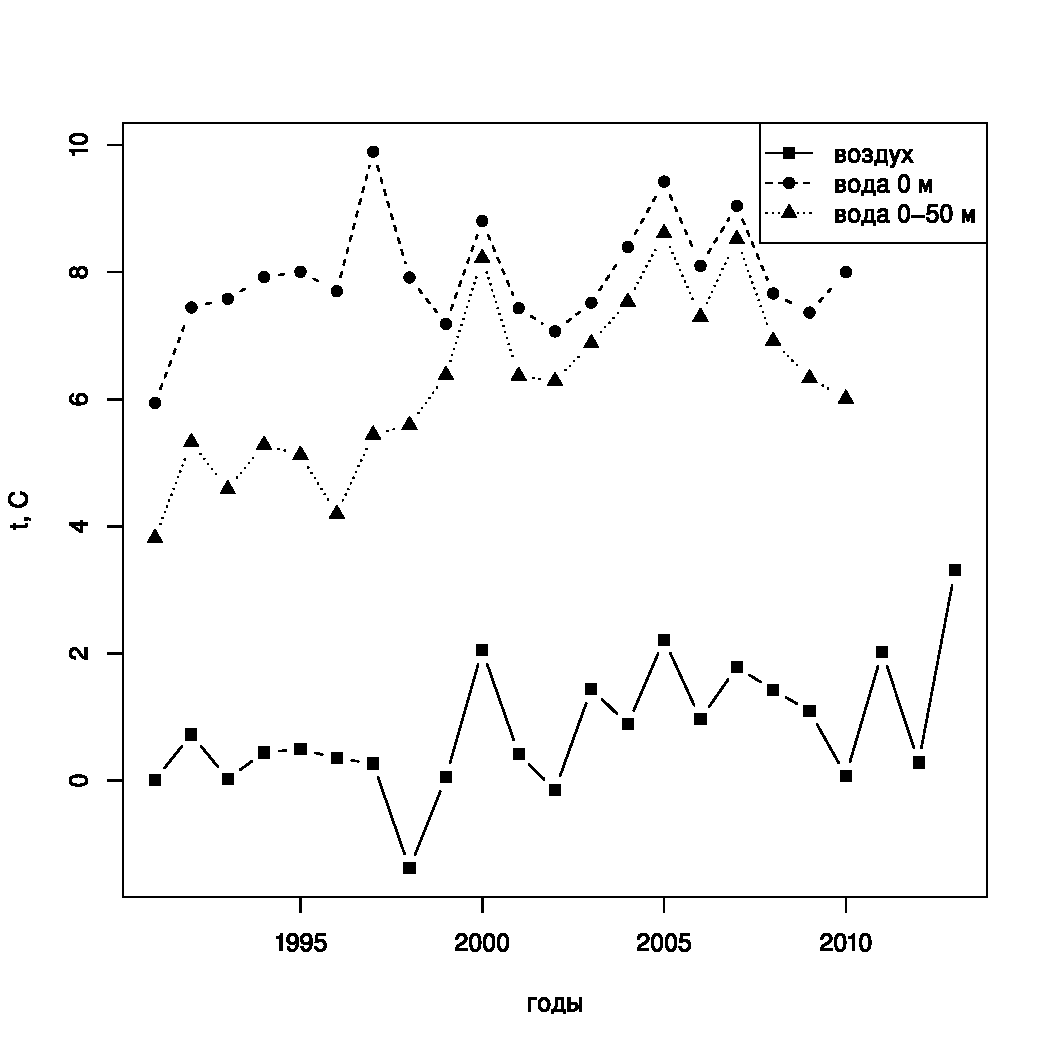
\includegraphics[width=\textwidth]{../temperatures_water_air/White_temp_air_water_dynamic1.pdf}
    \caption{Динамика среднегодовых температур воды и воздуха в Кандалакшском заливе Белого моря}
    \label{ris:White_temp_year_dynamic}
	\end{figure}

Среднегодовая температура воздуха и температура воды достоверно скоррелированы (корреляция Спирмена для температуры поверхности воды: $\rho = 0,3, p = 0,0035$, для температуры верхнего 50-метрового слоя: $\rho = 0,7, p = 0,0008$).


Использование среднегодовых значений температуры скрывает сезонное варьирование, которое может быть принципиально важно для поселений маком (например: \cite{Beukema_et_al_1998, Beukema_Dekker_2003, Beukema_et_al_2009}). 
Корреляция среднесезонных температуры воздуха и поверхности воды выше, чем среднегодовых значений (корреляция Спирмена для температуры поверхности воды: $\rho = 0,92, p < 0,0001$ (рис.~\ref{ris:White_temp_water_vs_air_seasons}. 
	\begin{figure}
    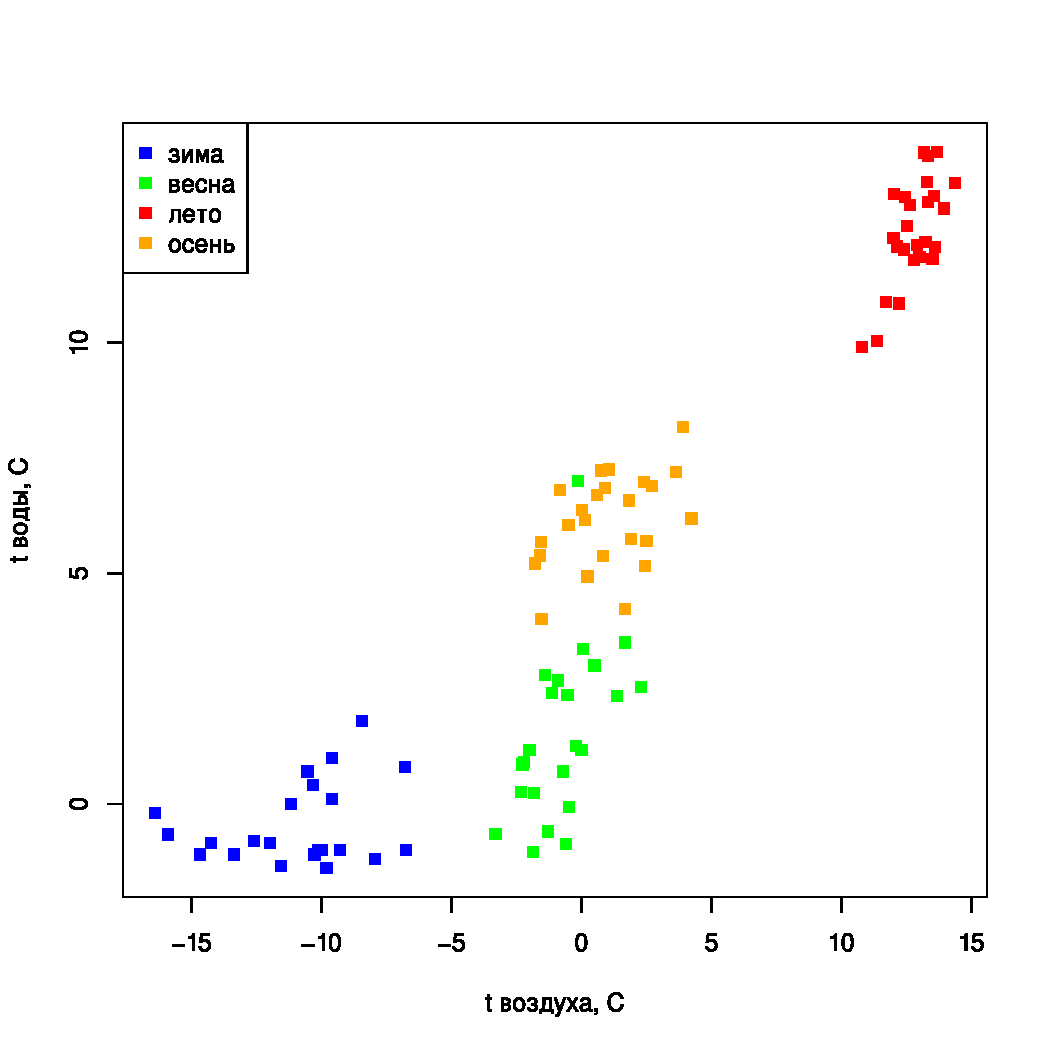
\includegraphics[width=\textwidth]{../temperatures_water_air/temp_air_water1.pdf}
    \caption{Соответсвие среднесезонных температур воды и воздуха в Кандалакшском заливе Белого моря}
    \label{ris:White_temp_water_vs_air_seasons}
	\end{figure}
Динамика средней температуры воды в разные сезоны представлена на рисунке~\ref{ris:White_temp_seasons_dynamic}.
	\begin{figure}
    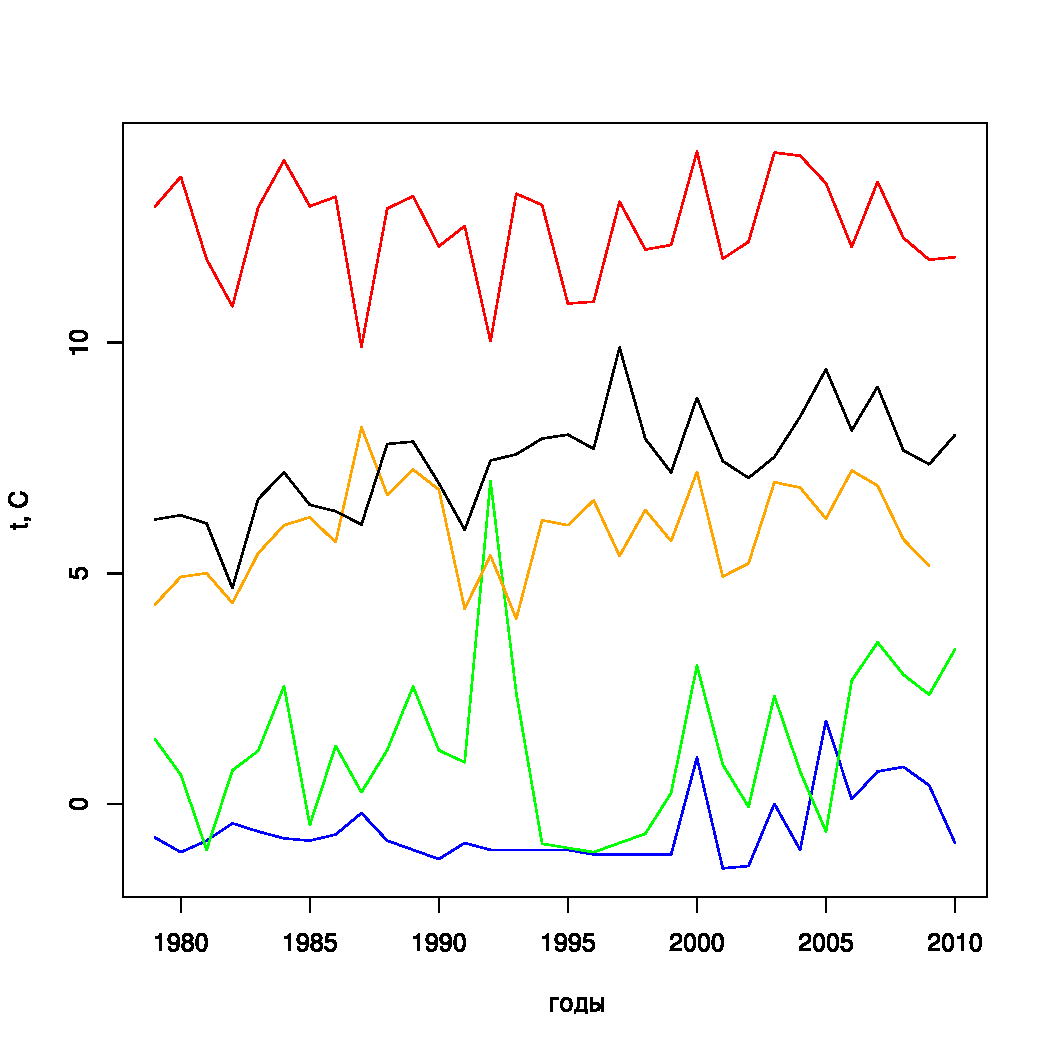
\includegraphics[width=\textwidth]{../White_Sea/temperature_Kartesh/t_mean_season_year1.pdf}
    \caption{Динамика среднесезонных температур воды и воздуха в губе Чупа(Кандалакшский залив Белого моря) (\cite{Berger_et_al_2003})}

{\footnotesize Примечание: t, C --- температура поверхности воды: синий --- зимняя, зеленый --- веснняя, красный --- летняя, оранжевый --- осенняя, черный --- среднегодовая. }
    \label{ris:White_temp_seasons_dynamic}
	\end{figure}

Очевидно, что локальные условия могут значительно варьировать в зависимости, например, от закрытости акватории, однако для оценки глобальных климатических воздействий мы считаем возможным использовать данные по Чупе для сравнения температурного режима в разные годы для всех участков в Кандалакшском заливе.




	\subsubsection{Баренцево море}

Баренцево море --- окраинное море, характерной особенностью гидрологического режима Баренцева моря является наличие двух  водных масс --- арктической (полярные воды, большую часть года покрытых плавучими льдами) и субарктической (субполярных вод, свободных от плавучих льдов) (\cite{Adrov_1992}). 

%Мурманским побережьем или Мурманом называют береговую линию Северного ледовитого океана от мыса Святой нос на востоке до реки Ворьемы на западе. 
%Данный район разделяют на несколько областей: Западный Мурман --- от реки Ворьемы до острова Кильдин или до Кольского залива, и Восточный Мурман --- далее на восток до мыса Святой нос (\cite{Derugin_1915}).

Постоянный подток теплых атлантических вод препятствует образованию льда вдоль Мурманского побережья, и он встречается главным образом во внутренних частях губ и заливов.
Несколько большее количество льда образуется ежегодно в юго-восточном районе Мурмана, в то время как по Западному Мурману, как правило, не образуется сплошного припая. 
В основном, исключая некоторые опресненные закрытые бухты и заливы, влияние морского льда на распределение животных невелико, гораздо большее значение зимой играет сильное промораживание литорали во время отлива (\cite{Propp_1971}).

Приливы на Мурмане являются правильными полусуточными и образуются единой атлантической приливной волной. 
Далее она распространяется вдоль Мурмана на восток до Новой Земли. 
Высота приливной волны составляет $3$ метра. 

В среднем, соленость вод у Мурманского побережья составляет $33,2 - 33,6$~\permil. 
Только весной во время сезонного увеличения берегового стока наблюдается краткое распреснение поверхностных слоев до $28 - 30$~\permil, однако толщина опресненного слоя не превышает $2 - 3$~м.

Кольский залив --- самый крупный из заливов Мурманского побережья Баренцева моря, лежит на границе Восточного и Западного Мурмана.
Географически в Кольском заливе выделяется три части, называемые коленами залива. 

Первое, северное или нижнее колено простирается от входа в Кольский залив до линии, соединяющей устье губы Средней и мыс Лас. 
Эта часть залива наиболее глубоководная (более $400$~м). 
Береговая линия северного колена Кольского залива чрезвычайно изрезана, и  здесь находятся самые крупные губы, в том числе Пала-губа, ставшая объектом наших наблюдений (\cite{Derugin_1915}).


Среднее колено (глубины до $200$~м) изогнуто в направлении к северо-западу и простирается на юг до мысов Пинагория и Мишукова. 
Второй участок наблюдений был расположен в районе границы северного и среднего колена Кольского залива (Ретинское).

Южная или верхняя часть наиболее мелкая (глубина около $50$~м), имеет направление с севера на юг, как и нижняя. 
В кут Кольского залива впадает две крупные реки --- Тулома и Кола, и одна более мелкая --- Лавна (\cite{Derugin_1915}).  
В районе самого узкого участка Кольского залива (Абрам-мыс) был расположен третий участок исследования в данном районе.
Последний участок, исследованный в Кольском заливе был расположен на западном берегу залива в черте города Мурманск (Северное Нагорное) в $3$~км от устья реку Туломы.

Воды Кольского залива неоднородны по своим свойствам. 
Это связано с несколькими причинами: большая протяженность залива, наличие глубоко вдающихся в побережье губ, влияние стока рек и ручьев. 
Гидрологическое лето начинается в поверхностных слоях воды в начале июля и продолжается до конца августа. 
Летом вода прогревается до $+ 8 - +18^{\circ}\ C$ в различных частях залива.

В  северном колене залива летом поверхностный слой значительно распреснен и соленость может достигать $8$~\permil, причем толщина распресненного слоя может достигать $3-4$~метров. 
Глубже соленость не опускается ниже $30$~\permil и у дна достигает $34$~\permil. 
Зимой соленость поверхностного слоя также составляет $30 - 34$~\permil. 

В южном колене в районе Абрам-мыса колебания солености на поверхности еще более заметны. 
Здесь сказывается не только сезонность стока, но и значительное влияние оказывает приливно-отливные течения. 
Летом во время прилива поверхностный слой толщиной до 3 метров обладает соленостью от $2$ до $16$~\permil, в то время как на глубине $3$~метра соленость колеблется в пределах от $28$ до $31$~\permil. 
В отлив мощность опресненного слоя увеличивается до $8$~метров, а поверхностная вода становится практически пресной (\cite{Derugin_1915}).

Таким образом, исследованные нами участки в Кольском заливе расположены в контрастных по географическим условиям его частях и позволяют относительно полно судить о данной акватории.

Фауна литораль Западного Мурмана наиболее богата по сравнению с остальным Мурманским побережьем. 
Традиционно, это связывают с более высокой среднегодовой температурой (температура воздуха в губах Западного Мурмана может быть на $0,4^{\circ}\ C$ выше по сравнению с Восточным Мурманом) и соленостью (выше $31$~\permil\ в поверхностном слое) и закрытости губ Западного Мурмана от основной акватории моря (\cite{Guryanova_et_al_1930}). 
К сожалению, данный регион оказался для нас малодоступен при исследованиях, и мы располагаем лишь данными об обилии маком в губах Ура и Печенга.
Однако данные губы расположены в разных частях Западного Мурмана, что позволяет нам делать предвательные выводы о данном регионе.

Береговая линия Восточного Мурмана менее изрезана, чем Западного Мурмана. 
Побережье большинства небольших заливов и губ не защищено от прибойного воздействия (\cite{Guryanova_Ushakov_1929}).
Таким образом, Восточный Мурман на большем его протяжении не является благоприятным для развития литоральных инфаунных сообществ, однако существуют глубоко вдающиеся в побережье бухты, в которых обнаруживается меньшее волновое воздействие. 
Именно на литорали таких губ и заливов и формируются наиболее богатые инфаунные сообщества данного региона, включающие {\it M.~balthica}.

Наши исследования охватывают Восточный Мурман на значительном его протяжении: $6$~участков от губы Гаврилово до губы Ивановская (длина береговой линии более $150$ километров).
Обследованные бухты варьируют по длине, степени изолированности и наличию в них ручьев и небольших рек, влияющих на локальное опреснение.


География исследований охватывает в том числе Дальний пляж губы Дальнезеленецкой --- исторически наиболее обследованной бухты на Мурмане.
Губа ДальнеЗеленецкая включает в себя две бухты --- бухта Оскара и бухта, в кутовой части которой располагается литоральная отмель Дальнего Пляжа. 
Важной характеристикой губы является изолированность ее от интенсивного волнового воздействия за счет наличия островов на входе.
	
При максимальных отливах протяженность литорали Дальнего пляжа с северо-запада на юго-восток составляет около $460$~м, а с юго-запада на северо-восток -- около $400$~м. 
	
В южной части отмели располагается дельта небольшого Зеленецкого ручья, вызывающего незначительное опреснение. 
Так, грунтовая вода, взятая у самого ручья, имеет соленость $32,9$~\permil, а взятая на два метра в стороне от ручья --- $34,07$~\permil (\cite{Prigorovskiy_1948}). 
Гидрологический режим характеризуется тем, что в бухту заходят воды из более глубоких и холодных слоев открытого моря, что вызывает уменьшение температуры и повышение солености (\cite{Voronkov_et_al_1948}).

Волновая активность в губе не превышает $1,5 - 2$ балла (\cite{Alexeev_1976}). 
Наиболее сильному волновому воздействию подвержена южная и юго-восточная части отмели, где на галечно-валунном пляже располагается зона штормовых выбросов.
Придонная скорость течений, вызванных приливной волной, составляет $0,8$~м/сек. при глубине 0,3-0,5 метров и 0,06 м/сек. при глубине более $2$~метров.

Для песчаных отмелей характерна только одна граница --- уровень высачивания, который делит пляж на две части, отличающиеся по условиям увлажненности донного осадка во время отлива (\cite{Streltsov_Agarova_1978}). 
Обширный, располагающийся ниже уровня высачивания и увлажненный во время отлива <<ватт>> простирается от отметок 1,25 до 2,1 м. над нулем глубин, сменяясь выше уровня высачивания узким $30$-метровым пляжем, где вода, занимавшая во время прилива интерстициальное пространство, вместе с грунтовыми водами вытекает на поверхность донного осадка. 
В западной части пляжа, самые верхние горизонты заняты валунной грядой (\cite{Agarova_et_al_1976}). 

Грунты отмели однообразны почти на всем ее протяжении. 
Мощность верхнего слоя ничтожна, и составляет $5 - 8$~см \cite{Prigorovskiy_1948}). 
Для отмели процессы размыва преобладают над накоплением. 
Даже в зоне относительно высокой аккумуляции, в <<языках>> дельты ручья, мощность голоценовых отложений составляет всего $15 - 30$~см.

Максимальная концентрация песков (более $90$\% по массе) отмечена в юго-восточной оконечности у подножья террасы, сложенной древними морскими песками. Еще одной особенностью пляжа является повышенное содержание алевропелитов (\cite{Pavlova_1976}). 
Их локализация на пляже обусловлена эрозивной волноприбойной деятельностью, доминирующей при среднем уровне малой воды (\cite{Alexeev_1976}).

Органическое вещество представлено гумусовыми соединениями и битумоидами местного и континентального происхождения (\cite{Gurevich_Yakovleva_1976}).
Наши мониторинговые работы в губе Дальнезеленецкая продолжают череду количественных гидробиологических исследований данного района (\cite{Prigorovskiy_1948, Matveeva_et_al_1955, Streltsov_et_al_1974, Agarova_et_al_1976, Zhukov_1984}).


Таким образом, выбранные участки достаточно разнообразны по своей географической приуроченности и связанных с ней абиотических градиентов (температура и соленость).

		\paragraph{Динамика температур}
Для Баренцева моря доступны данные по динамике температур на разрезе Кольский меридиан (\cite{pinro}). 
Наиболее адекватными данными для оценки динамики литоральных температурных условий представляются данные о средней температуре в верхнем 50-метровом слое воды на прибрежных станциях (рис.~\ref{ris:Barents_temp_dynamic}).
	\begin{figure}
    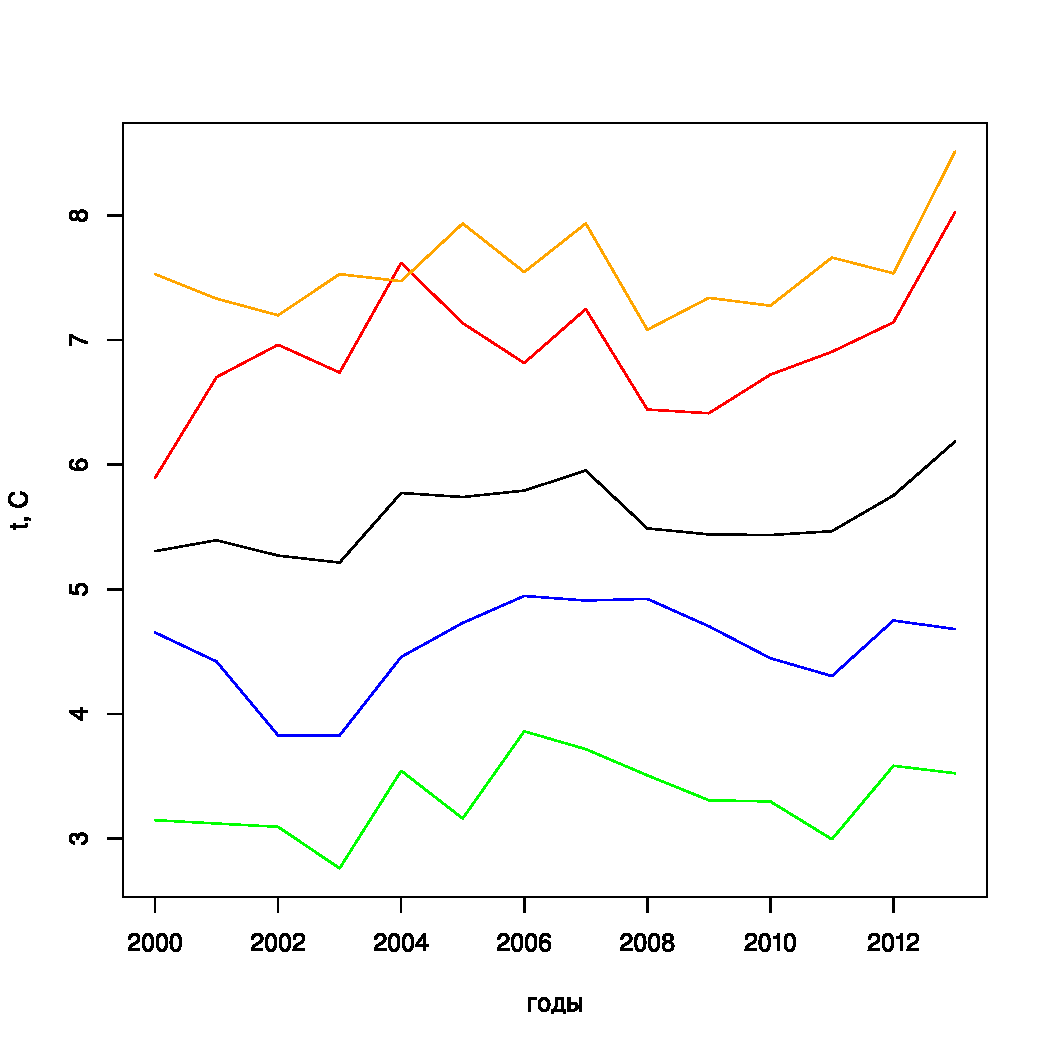
\includegraphics[width=\textwidth]{../Barenc_Sea/temperature/t_air_mean_season_year1.pdf}
    \caption{Динамика температуры воды верхнего 50-метрового слоя на разрезе Кольский меридиан(станции 1-3) (\cite{pinro})}

{\footnotesize Примечание: t, C --- температура поверхности воды: синий --- зимняя, зеленый --- веснняя, красный --- летняя, оранжевый --- осенняя, черный --- среднегодовая. }
    \label{ris:Barents_temp_dynamic}
	\end{figure}


\vspace{2cm}

Таким образом, условия обитания маком в Белом и Баренцевом море различаются по многим параметрам.
Температурный режим прибрежной части Кандалакшского залива Белого характеризует более значительные сезонные колебания(рис.~\ref{ris:temp_White_Barents}).
	\begin{figure}
    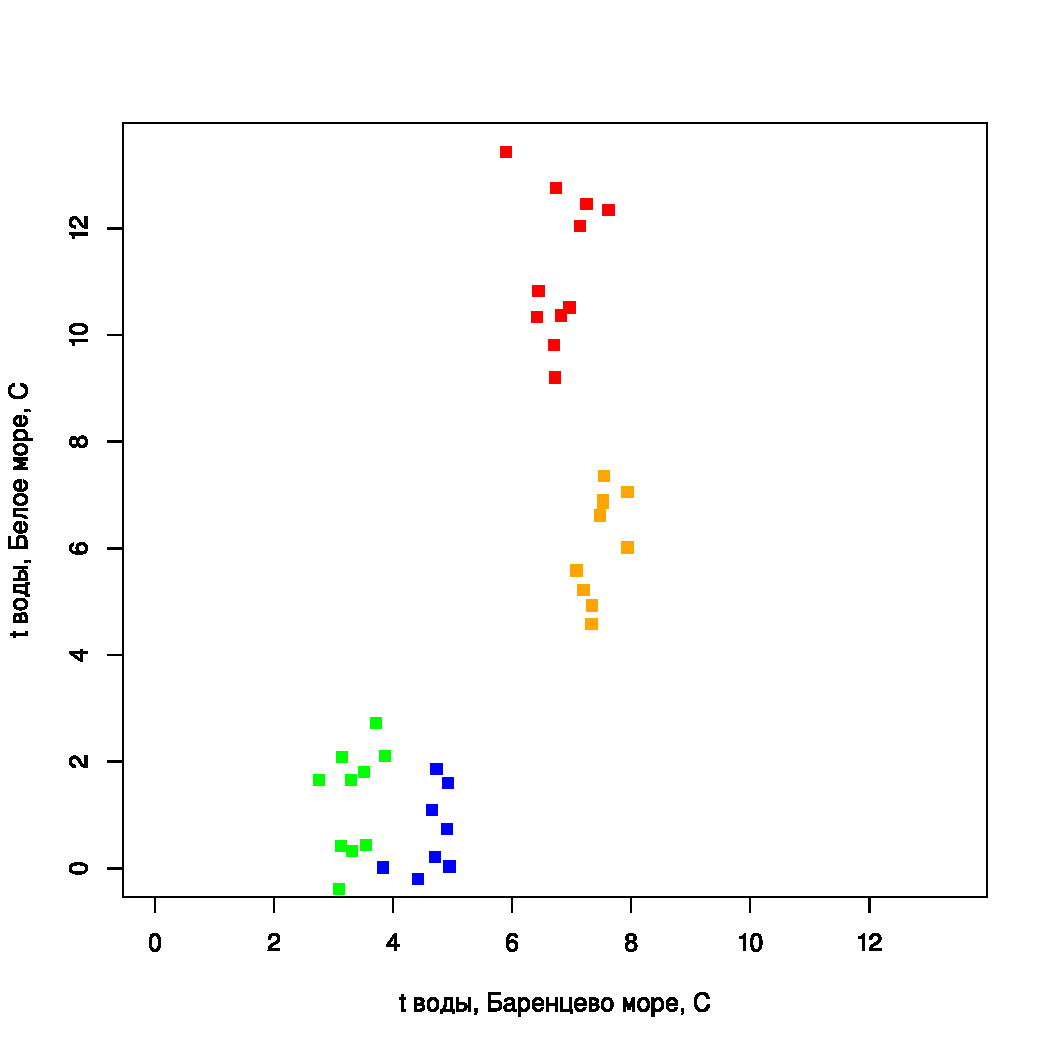
\includegraphics[width=\textwidth]{../temperatures_water_air/temp_White_Barents1.pdf}
    \caption{Соотношение среднесезонных температур в верхнем 50-метровом слоях воды в Белом и Баренцевом морях}

{\footnotesize Примечание: t, C --- температура поверхности воды: синий --- зимняя, зеленый --- веснняя, красный --- летняя, оранжевый --- осенняя}
    \label{ris:temp_White_Barents}
	\end{figure}
В пределах каждого сезона межгодовые изменения в Белом море также выше, чем в Баренцевом.
Кроме того, различается сезонность хода температур. 
В Белом море лето является наиболее теплым сезоном, а зима --- наиболее холодным.
Для Баренцева моря гидрологическая сезонность сдвинута относительно календарной: самый теплый сезон это осень, а самый холодный --- весна.

Данные о солености в маштабах крупных акваторий не очень показательны для бентосных огранизмов, поскольку локальные условия, например, наличие берегового стока в данном месте, значительно меняют данный показатель. 
Кроме того, соленостная толерантность {\it M.~balthica} достаточно высока (\cite{***}), хотя данный вид считается эстуарным (\cite{***}). 
Однако для беспозвоночных с планктонной личинкой, как у макомы, общая соленость в акватории может играть роль.
В целом, исследованный район в Баренцевом море характеризуется соленостью близкой к океанической.
Характерно, что все поселения на Западном и Восточном Мурмане расположены в губах, в которые впадают небольшие реки или ручьи, то есть находятся в распресненных условиях.
Соленость в Кольском заливе ниже океанической за счет впадения в кут залива крупных рек Колы и Туломы, и таким образом участки, расположенные вне губ с локальным стоком, тоже находились в распресненных условиях.
Тем не менее, невозможно утверждать, что распределение маком на Мурмане находится под влиянием солености, так как невозможно изолировать несколько важных абиотических фактора: соленость, характер грунта и степень прибойности/закрытости акватории. 
Поскольку для Мурманского побережья характерно наличие берегового стока в закрытых губах (\cite{Guryanova_Ushakov_1929, Guryanova_et_al_1930}).
Белое море в целом характеризуется пониженной соленостью и среднегодовая не превышает 25~\permil.
В данной акватории нельзя говорить о приуроченности поселений маком в локальному береговому стоку, и среди исследованных участков были как участки, находящиеся под влиянием рек и ручьев, так и вне зоны влияния оных.

\textcolor{red}{ГРУНТЫ}

%%%%%%%%%%%%%%%%%%%%%%%%%%%%%%%%%
%макома как типичный компонент литоральных сообществ.? Гурьянова и Ко - в Баренцевом. Белое - ээээ.
		\subsection{{\it Macoma balthica} как массовый элемент в сообществах литорали северных морей}

%MsC
Моллюски {\it M.~balthica} --- типичные обитатели илисто-песчаной литорали умеренной зоны Северного полушария. 
В Баренцевом море макомы вместе с другими представителями бореальной и бореально-арктической фауны заселяют пляжи осушной зоны в верхней сублиторали. 
Судя по описаниям состава сообществ организмов макробентоса в изученных местообитаниях мы имели дело с типичными для Баренцева моря биосистемами. 
Все отмеченные нами виды характерны для литорали Кольского залива и Восточного Мурмана (\cite{Derugin_1915, Guryanova_Ushakov_1929}).



%%%%%%%%%%%%%%%%%%%%%%%%%%%%%%%%%
%структура поселений маком.


%%%%%%%%%%%%%%%%%%%%%%%%%%%%%%%%%
%Обилие макомы - соотношение наших данных и литературных по нашим регионам. обилие макомы в разных частях ареала. не работает гипотеза что в центре много.
		\subsection{Обилие {\it Macoma balthica} в европейской части ареала}
Традиционно считается, что {\it M.~balthica} амфибореальный вид. 

В Атлантическом океане данный вид встречаются по всему европейскому побережью до Франции на юге. 
По американскому --- от штата Джорджия на юге до моря Баффина и западного побережья Гренландии на севере. 
В Тихом океане {\it M.~balthica} встречается до залива Посьет в Японском море по азиатскому берегу, и до Сан-Диего --- по американскому. 
Также данный вид заходит в моря Северного Ледовитого океана:  Норвежское, Баренцево, Белое, Карское, Чукотское и Бофорта. 
В западном секторе Арктики, самые восточные находки вида --- из Байдарацкой губы Карского моря, а самые северные --- со Шпицбергена (\cite{Semenova_1974, Kafanov_1985, Maximovich_1985, Meehan_1985, Naumov_Skorobogatov_1987, Meehan_et_al_1989, Hummel_et_al_1997}).

Современные молекулярные исследования показывают неоднородность вида {\it M.~balthica} sensu lato в пределах ареала, причем можно говорить о нескольких уровнях гетерогенности. 
Рассматривая самый верхний уровень внутривидовой генетической структуры, в настоящее время предлагают выделять атлантический ({\it M.~balthica rubra} и тихоокеанский {\it M.~balthica balthica} подвиды.
Однако  в морях, связанных с  Атлантикой, существуют очаги распространения тихоокеанской формы. 
Так, в Балтийском, Белом и Баренцевом морях обитает тихоокеанская форма {\it M.~balthica balthica}. В Баренцевом море она распространена на восток до Варангер-фьорда (\cite{Vainola_2003}). 

Мы рассматривали полученные нами данные об обилии маком в Белом и Баренцевом морях в контексте литературных данных об обилии данного вида в европейской части ареала.


%MSc
По нашим данным, на литорали Кольского залива численность {\it M.~balthica} составляла около $1000$~экз./м$^2$, что хорошо соотносится с результатами, полученными ранее для других областей данной акватории. 
Так, обладая данными по большему количеству участков, Л. Басова приводит средние показатели плотности поселения маком $802 \pm 273$~~экз./м$^2$ при максимальной численности $2900$~экз./м$^2$ (Басова, 2004, Генельт-Яновский и др., 2005В). 
Для более южных акваторий (Белое, Северное, Балтийское моря) столь высокое обилие данных моллюсков также является характерным (Segerstrale, 1960; Семенова, 1974; Максимович и др., 1991, Strasser et al., 2003; Назарова, Полоскин, 2005). На Восточном Мурмане численность M. balthica в основном не превышала 100 экз/м2, лишь на одном участке достигая 500 экз/м2. В принципе, такие низкие численности маком отмечены и для других частей ареала (Басова, 2004; Strasser et al., 2003), однако обычно низкие значения обилия присутствуют лишь как одна из стадий динамики поселения. В данном же случае есть основания предполагать, что столь низкие значения показателей обилия устойчивы во времени. Так, в губе Дальне-Зеленецкой в течение 7 лет (то есть в течение времени, сравнимым со средней продолжительностью жизни моллюсков — 8-10лет) плотность поселения	оставалась менее 70 экз/м2 и была сопоставима с данным показателем в 1974 году. 
	Л. Басовой для Кольского залива была показана достоверная положительная корреляция между численностью M. balthica и содержанием органических веществ в грунте (Басова, 2004).   Однако для полученных нами данных такая закономерность не обнаружена. В то же время, по нашим данным численность маком достоверно коррелировала с долей песчаный фракций. Была показана прямая связь с мелким песком и обратная — с крупным. Характеристики грунта важны для моллюсков с одной стороны на субстрат для обитания, а с другой — как источник пищи. Обычно предполагается, что предпочтение особями более мелкодисперсных грунтов связано с более высокой концентрацией органических веществ в таком грунте. Хотя часто концентрация органических веществ положительно коррелирует с долей мелкого песка и алевро-пеллита (Бубнова, 1972; Басова, 2004), для исследованных участков на статистическом уровне этого не показано, хотя и наблюдается тенденция к этому. 	Показано (Olaffson, 1989), что на песчаном грунте M. balthica начинают питаться не как собирающие детритофаги, а как фильтраторы. Таким образом, основную роль начинают играть не органические вещества в осадках, растворенные в воде. В таком случае наличие в Кольском заливе поселков и городов, в которых есть бытовые стоки, может объяснять более высокое обилие маком именно в данной акватории.

%%%%%%%%%%%%%%%%%%%%%%%%%%%%%%%%%
%скорость роста в разных частях ареала. Букма-Меган - врисовать наши точки в их картинку...



%%%%%%%%%%%%%%%%%%%%%%%%%%%%%%%%%
%динамика поселений

